%!TEX root = ../Masterthesis.tex
\chapter{System Evaluation}
\begin{figure}[H]
\centering
\includegraphics[width=0.9\textwidth]{images/complete_setup.png}
\caption{Final system setup with cameras on construction profile, color markers and visualization.}
\label{img:complete_setup} 
\end{figure}
\section{Camera hardware and control}
The Raspberry Pi image processing of the camera frames can be a significant bottleneck for the system. "Real-time" evaluation demands the processing time of a frame to be in the range of the time of the camera FPS to utilize all available frames. With the current system setup limited to 30 fps by the camera framework, the image processing has to be done in about $1/30s$ or 33 ms to achieve "real-time" processing. Professional stereoscopic setups use cameras with global shutters and a synchronization signal. This enables a sub-frame synchronization of the two camera systems. The cameras used in the prototype setup use a rolling shutter instead. Furthermore, these cameras are designed to be of easy use for the normal consumer, therefore their design does not incorporate a synchronization feature. To achieve a form of hardware synchronization, a large amount of reverse engineering would be needed as the electrical drawings as well as the controlling software are closed source. The multi-layered circuit board of the camera would also complicate the reverse engineering step.  For these reasons, attempting the synchronization of the data further down the processing pipeline was more reasonable.
\\To synchronize the  frame reading of both cameras, the system boots up to the point where all needed components are initialized. At this point, the program waits for a start message from the "Master" system via \textit{UDP}. The "Master" system send the start message at the end of its initialization phase via a \textit{UDP} broadcast.This ensures that both Raspberry's get the message at the same time.
In normal usage mode, the camera uses automatic modes for it's parameter setup. This continuous measuring mode produced fluctuation in image brightness and color saturation. To eliminate this problem, all automatic modes were turned off in the camera initialization phase. Fixed values are loaded from a \textit{JSON} file instead. To get the values for the \textit{JSON} file, a calibration step was implemented. This calibration step enables the user to preview and manipulate the following values for the camera:
\begin{itemize}
\item Saturation
\item Brightness
\item Gain
\item Exposure time
\item Contrast
\item White balance values for blue and red channel
\end{itemize}
\begin{figure}[H]
\includegraphics[width=\textwidth]{images/calib_windows.jpg}
\caption{Camera and color calibration utility window}
\label{fig:calibration_windows} 
\end{figure}
The user-set calibration values can be written into a new \textit{JSON} file. They are directly loaded into the program after calibration is finished. Control over these parameters showed to be crucial for achieving a constant color separation. The threshold values for the color tracking also needed to be initially calibrated. These values are dependent on the lighting situation and any change results in the need for re-calibration. To simplify this calibration, a calibration functionality in line with the camera calibration was implemented. The implemented feature provides the user with a preview of the resulting thresholded black and white image with applied camera settings. Range sliders for lower and upper boundaries for the three RGB components make it fairly easy to adjust and view thresholding results in "real-time". The calibration values can also be stored into a \textit{JSON} file. This file can then be read out on following program start-ups.
\section{Image processing performance}
The first prototype implementation with \textit{OpenCV} in \textit{Python} showed, that a speed of 33 ms was achievable when only tracking one color. The implementation reached around 30 - 40 ms processing time when scanning whole images. An implementation of an \textit{"Region of interest"} feature reduced the processing time to around 30 ms for a single color. The downside of the implementation was revealed when implementing the other 4 colors needed to do a full five finger tracking. This approach ramped-up processing time to around 100 ms per frame, making this solution run at 10 FPS.\\\\ 
The sequential algorithm also showed another design flaw. When not utilizing the ROI approach, the algorithm would scan the whole grabbed camera frame for each color to create the corresponding threshold map. The \textit{OpenCV} color threshold methods are designed to only search for one color threshold at the time. They therefore need this procedure. One solution option is the already mentioned data reduction through ROI usage. This solution could furthermore benefit from a multi-threaded implementation. The original image data is only read. Parallel memory readout is not a problem and the generated mask can be saved separately.\\
\\Another approach which could help speed up the process is implementing an own method for thresholding the grabbed frame. This would result in the possibility to do all the needed color thresholds in one image loop. With this solution, the overhead would be reduced by 4 image iterations. The thresholding operations would stay the same as these still have to be run on each pixel. The output of this method would then return the 5 needed threshold mask for further processing.\\\\
A second performance issue that arose from the first prototype was that the input camera frames are RGB coded. For better options of color separations, the image was initially intended to be converted into HSV colorspace. This operation turned out to be second longest operation after frame grabbing. \\Testing of the cameras indicated that the color separation in the original RGB images of the cameras is good enough for the used test colors. This caused this step to be omitted and shaved off several milliseconds of processing time.
The rest of the processing steps are performed in the sub-millisecond range and are therefore not as valuable for performance optimization.
\\The results from this prototype indicated, that the \textit{OpenCV-Python} combination is not suitable for reaching the 30 ms target time. The OpenCV library used by python is actually just the ported version of the C code library with bindings for python. As \textit{C} and \textit{C++} are more hardware near and therefore more performant, a second prototype implementation was done in \textit{C++}.
\\\\The recreated workflow of the Python code in\textit{ C++} initially showed similar performance measurements when using a sequential approach. This was to be expected, as it is the same code the Python bindings are using. Further investigation into code timings showed, that another bottleneck was the image optimization feature which applied erosion and dilation operations to remove high frequency noise in the image. This operation brought the time up to 100 ms processing time when processing the whole frame area.This  makes the implementation not usable for "real-time" application. Removing this feature when scanning full frames resulted in a major speed up of processing time. \\
The implementation of a thread pool, which handles all the color detection jobs, brought down the calculation time for 5 colors to around 120-140 ms. Although these times are still not usable for real time, it brought a significant performance boost. Figure \ref{c++ work flow map} shows the initial structure design of the program with a camera frame buffer and the thread pool approach. The cyclic buffer was intended to hold images frames for readout where camera frame rates are much higher than the achieved processing rates of the source code.Since the frame-rates of the current setup are slower than the time spend on processing, the image-buffer for the camera is not needed. The feature is left in the code but is not actively used at the moment.\\
\\\\Since the thread pool approach still took too long, a test with lower resolution than 640x480 was done and showed that the calculation time can be reduced. This indicated that the ROI idea would be feasible for further performance optimization. A test at a frame resolution of 320x240 pixels reduced the processing time for all five colors to below 10 ms.\\Utilization of the knowledge from these tests led to the implementation of the aforementioned\textit{ "Region of interest"} feature.
The first frame is analyzed as a whole frame, optimally resulting in the detection of a marker. As the marker detection creates a rectangle around the tracked area, we already have the coordinates for the ROI and only have to add an offset to this area.
\\The value of the ROI offset has to be set high enough to ensure that in the following frame, the tracking marker is still contained. It also has to be ensured, that the generated ROI is clamped to the frame dimensions. If not doing so, parts of the readout are can be located outside of the image plane, causing readout errors when used for the subsequent frame.
\\The following frames will then be processed with the input of the ROI, selecting only the defined section of the image and updating the ROI with the new data for that frame. The \textit{C++} implementation brought down the processing time as assumed. This made it possible to apply the image improvement operations that were left out on the python implementation.
\\Performance measurement for tracking consistency with stationary color trackers was performed for a time period of 10.000 frames to get qualitative results. 
A sequential implementation with the usage of the ROI and image optimization was used for better analysis options and showed an average processing time of 46 ms with a standard deviation of ~11 ms.\\
\begin{figure}[H]
\centering
\includegraphics[width=\textwidth]{images/pi_workflow_500.jpg}
\caption{Intended work-flow of the C++ implementation with thread pool solution and ROI for high frame-rate solutions}
\label{c++ work flow map} 
\end{figure}

Further analysis showed that the high standard deviation came from peaks in performance times that took up to 400 ms when loosing tracking.\\ Filtering all values over 50 ms out from the data set showed that only $1\%$ ($\sim 1000$ out of $10.000$ frames) of the recorded processing times were lying outside of this time frame. Filtering out these values form the data set and recalculation dropped the average processing time down 3 ms to around 43 ms. The standard deviation was dropped drastically from its previous 11 ms to around $1.6$ ms. This shows that a filtering of processing times on the Raspberry could lead to a more consistent frame processing time. To do so, after every processing cycle the time should be checked. If it is over the defined time limit, no data should be sent.\\
Since this performance measurement does not give deeper insights on which part of the process consumes large amounts of processing time, the same measurement was done with a finer time tracking on the single parts of the processing pipeline.
\begin{table}[H]
\centering
\caption{Measurement results for sequential processing timing}
\label{tbl:sequential_performance_values}
\begin{tabular}{|c|c|c|c|c|c|}
\hline
\begin{tabular}[c]{@{}c@{}}Time \\ in ms\end{tabular} & \begin{tabular}[c]{@{}c@{}}Image \\ retrieval\end{tabular} & \begin{tabular}[c]{@{}c@{}}Stereo \\ rectification\end{tabular} & \begin{tabular}[c]{@{}c@{}}Color detection\\ (6 colors)\end{tabular} & \begin{tabular}[c]{@{}c@{}}UDP \\ sending\end{tabular} & \begin{tabular}[c]{@{}c@{}}Summed \\ time\end{tabular} \\ \hline
Average                                               & 0.92                                                  & 31.39                                                       & 14.55                                                             & 0.12                                                & 46.97 \\ \hline
Std.Deviation                                        & 0.17 & 7.19 & 5.06 & 0.06                                                & 10.77                                               \\ \hline
\end{tabular}
\end{table}
Table \ref{tbl:sequential_performance_values} highlights the performance bottlenecks of the system. Image retrieval from the camera as well as the time to process and send the data results via UDP are in the sub millisecond range. Therefore they impose no significant delay. Without these two steps, the remaining 96\% of the processing time is taken up by the image stereo rectification and the color tracking. When comparing these two, the far larger time consuming part is taken up by the stereo rectification part with nearly two thirds of the processing time.\\
The use of the stereo rectification in the system was done to ensure that the two used images have an aligned horizontal orientation. This is needed for camera pairs that are not aligned horizontally and/or parallel. Since the camera mounting ensures that the cameras are aligned parallel and at the same horizontal height, the rectification step can be omitted for performance reasons. It cuts down 67\% of the processing time of the system. As the stereo calculation does not use the vertical position difference for calculations, the possible resulting differences can be dealt with via filtering on the receiver side.
A solution for the color tracking time improvement was already described before. Utilizing a multi-threaded approach could lead to further reduction of the processing time.\\\\ A comparison between the before mentioned sequential algorithm with ROI and a multi-threaded implementation with ROI was tested as well. The multi-threaded implementation was designed to run the same processing stack as one loop of the sequential approach on each thread. Measurements over 10.000 frames for stationary as well as moving targets were made. One camera was run with the sequential implementation, while the second one ran the multi-threading approach. Thereby it is ensured that both cameras have the same measurement conditions.\\
The comparison of the measurements showed that in the current implementation state, the multi-threaded approach seems to have a much longer processing time. 
\begin{table}[h]
\centering
\caption{Measurement values of implementation comparison}
\label{tbl:implementaion_comparison}
\begin{tabular}{|l|l|l|}
\hline
Measurement            & Average (ms) & Std. Dev (ms) \\ \hline
Single-thread static  & 16.96        & 4.03          \\ \hline
Multi-thread static   & 32.09        & 10.64         \\ \hline
Single-thread dynamic & 19.41        & 22.44         \\ \hline
Multi-thread dynamic  & 35.80        & 22.88         \\ \hline
\end{tabular}
\end{table}
Table \ref{tbl:implementaion_comparison} shows that the measured time are roughly twice as long as the code running on a single thread. This behavior may result from an design or implementation fault in the multi-thread code and should be evaluated in future works to improve processing performance of the system. For the current state of the prototype, the single-threaded implementation with it's average processing time of around 19 ms is sufficient.
\newpage
\subsection{Color accuracy and ROI size}
As already mentioned in the conceptional phase, the lighting of the tracking area is a major factor. Variations of lighting intensity and color temperature cause the color of the trackers to shift their color. This can cause a fluctuation in the calculated tracker positions, as the defined color threshold ranges are kept as small as possible. This was done to achieve a clean separation of the tracker colors and reduce unwanted noise. \\\\
System testing with the 5 different colored shrink tubing markers proved, that the color tracking for colors outside of the color range of the human skin tones (green,blue) is rather unproblematic. The color markers falling into the colorspace of possible light reflection from skin may cause problems, depending on the lighting situation of the setup.
\begin{figure}[H]
\includegraphics[width=\textwidth]{images/color_tracking_probs.png}
\caption{Images showing reflection problems with  orange color thresholding. a) Correct threshold with only the marker being thresholded b-c) Depending on the rotation of the hand, skin reflection color falls into tracking threshold.}
\label{img:Color_reflecton_problems} 
\end{figure}
Figure \ref{img:Color_reflecton_problems} displays such a case where depending on the orientation of the hand, reflection from the scenery lighting can fall into the color tone space of the tracked marker. This can cause large parts of the hand to light up in the image. Since the calculation of the tracking marker position relies on finding the largest closed "white" area in the thresholded image, this can cause a "jumping" of the calculated position. 
\\\\The first solution for this problem is to narrow down the color threshold spans. By doing so, one can ensure that only the wanted colors are tracked. This method does have a downside effect. When the markers are moved in the tracking space, light variations and shadowing will cause the colors to shift their appearance slightly. With broader threshold ranges, this does not seem to be a large problem as these changes still lie inside the ranges. Narrowed down color ranges might not include these color variations. It could also create cavities in the thresholded image.\\ The applied morphological operations on the image can fix these problems up to a certain point, depending on filter kernel size, but for larger areas this could vary position tracking results.\\\\The implemented ROI feature speed up the whole system calculations once the colors are found. Before this point, the system scans whole frames to find colors, which takes more time than the much smaller ROI regions.
Empirical evaluations showed, that for the used tracking space, a ROI region size offset of 40 px in x and y directions produces the best results in terms of consistency. Smaller region offsets caused the system to use tracking for faster hand motion, which causes system slow down until the tracking has recovered. Larger ROI's showed to produce more consistent tracking results at the cost of higher calculation time.
\subsection{Finger markers}
\begin{wrapfigure}[19]{r}{0.3\textwidth} 
\centering
\includegraphics[width=0.5\textwidth,angle=-90]{images/color_markers_hand.jpg}
\caption{First set of shrink tube color markers }
\label{img:first_set_color_markers}
\end{wrapfigure}
The initial color marker size was selected to be relatively large, spanning most of the last segment size of each finger.
The used material of the colored shrink tubing was selected because it seemed to be relatively diffuse and therefore unsusceptible to errors resulting from the reflection of the scene lighting. The material turned out to be mostly diffuse reflecting, but depending on color and angle of light incidence, reflections in the color of the scene light did occur. A test-set of smaller markers was also evaluated, showing the same color reflection problems.\\The benefit of a smaller marker size would be much lower restriction of the finger movements and also unveiling the fingertips for better haptic interaction.
\\\\As both markers showed the above described problem of mixing marker area with possible skin reflections, an improvement to the markers was applied. At both ends of the larger markers, a piece of gray colored tape was applied to create an artificial border for the tracking algorithm.
\begin{figure}[H]
\centering
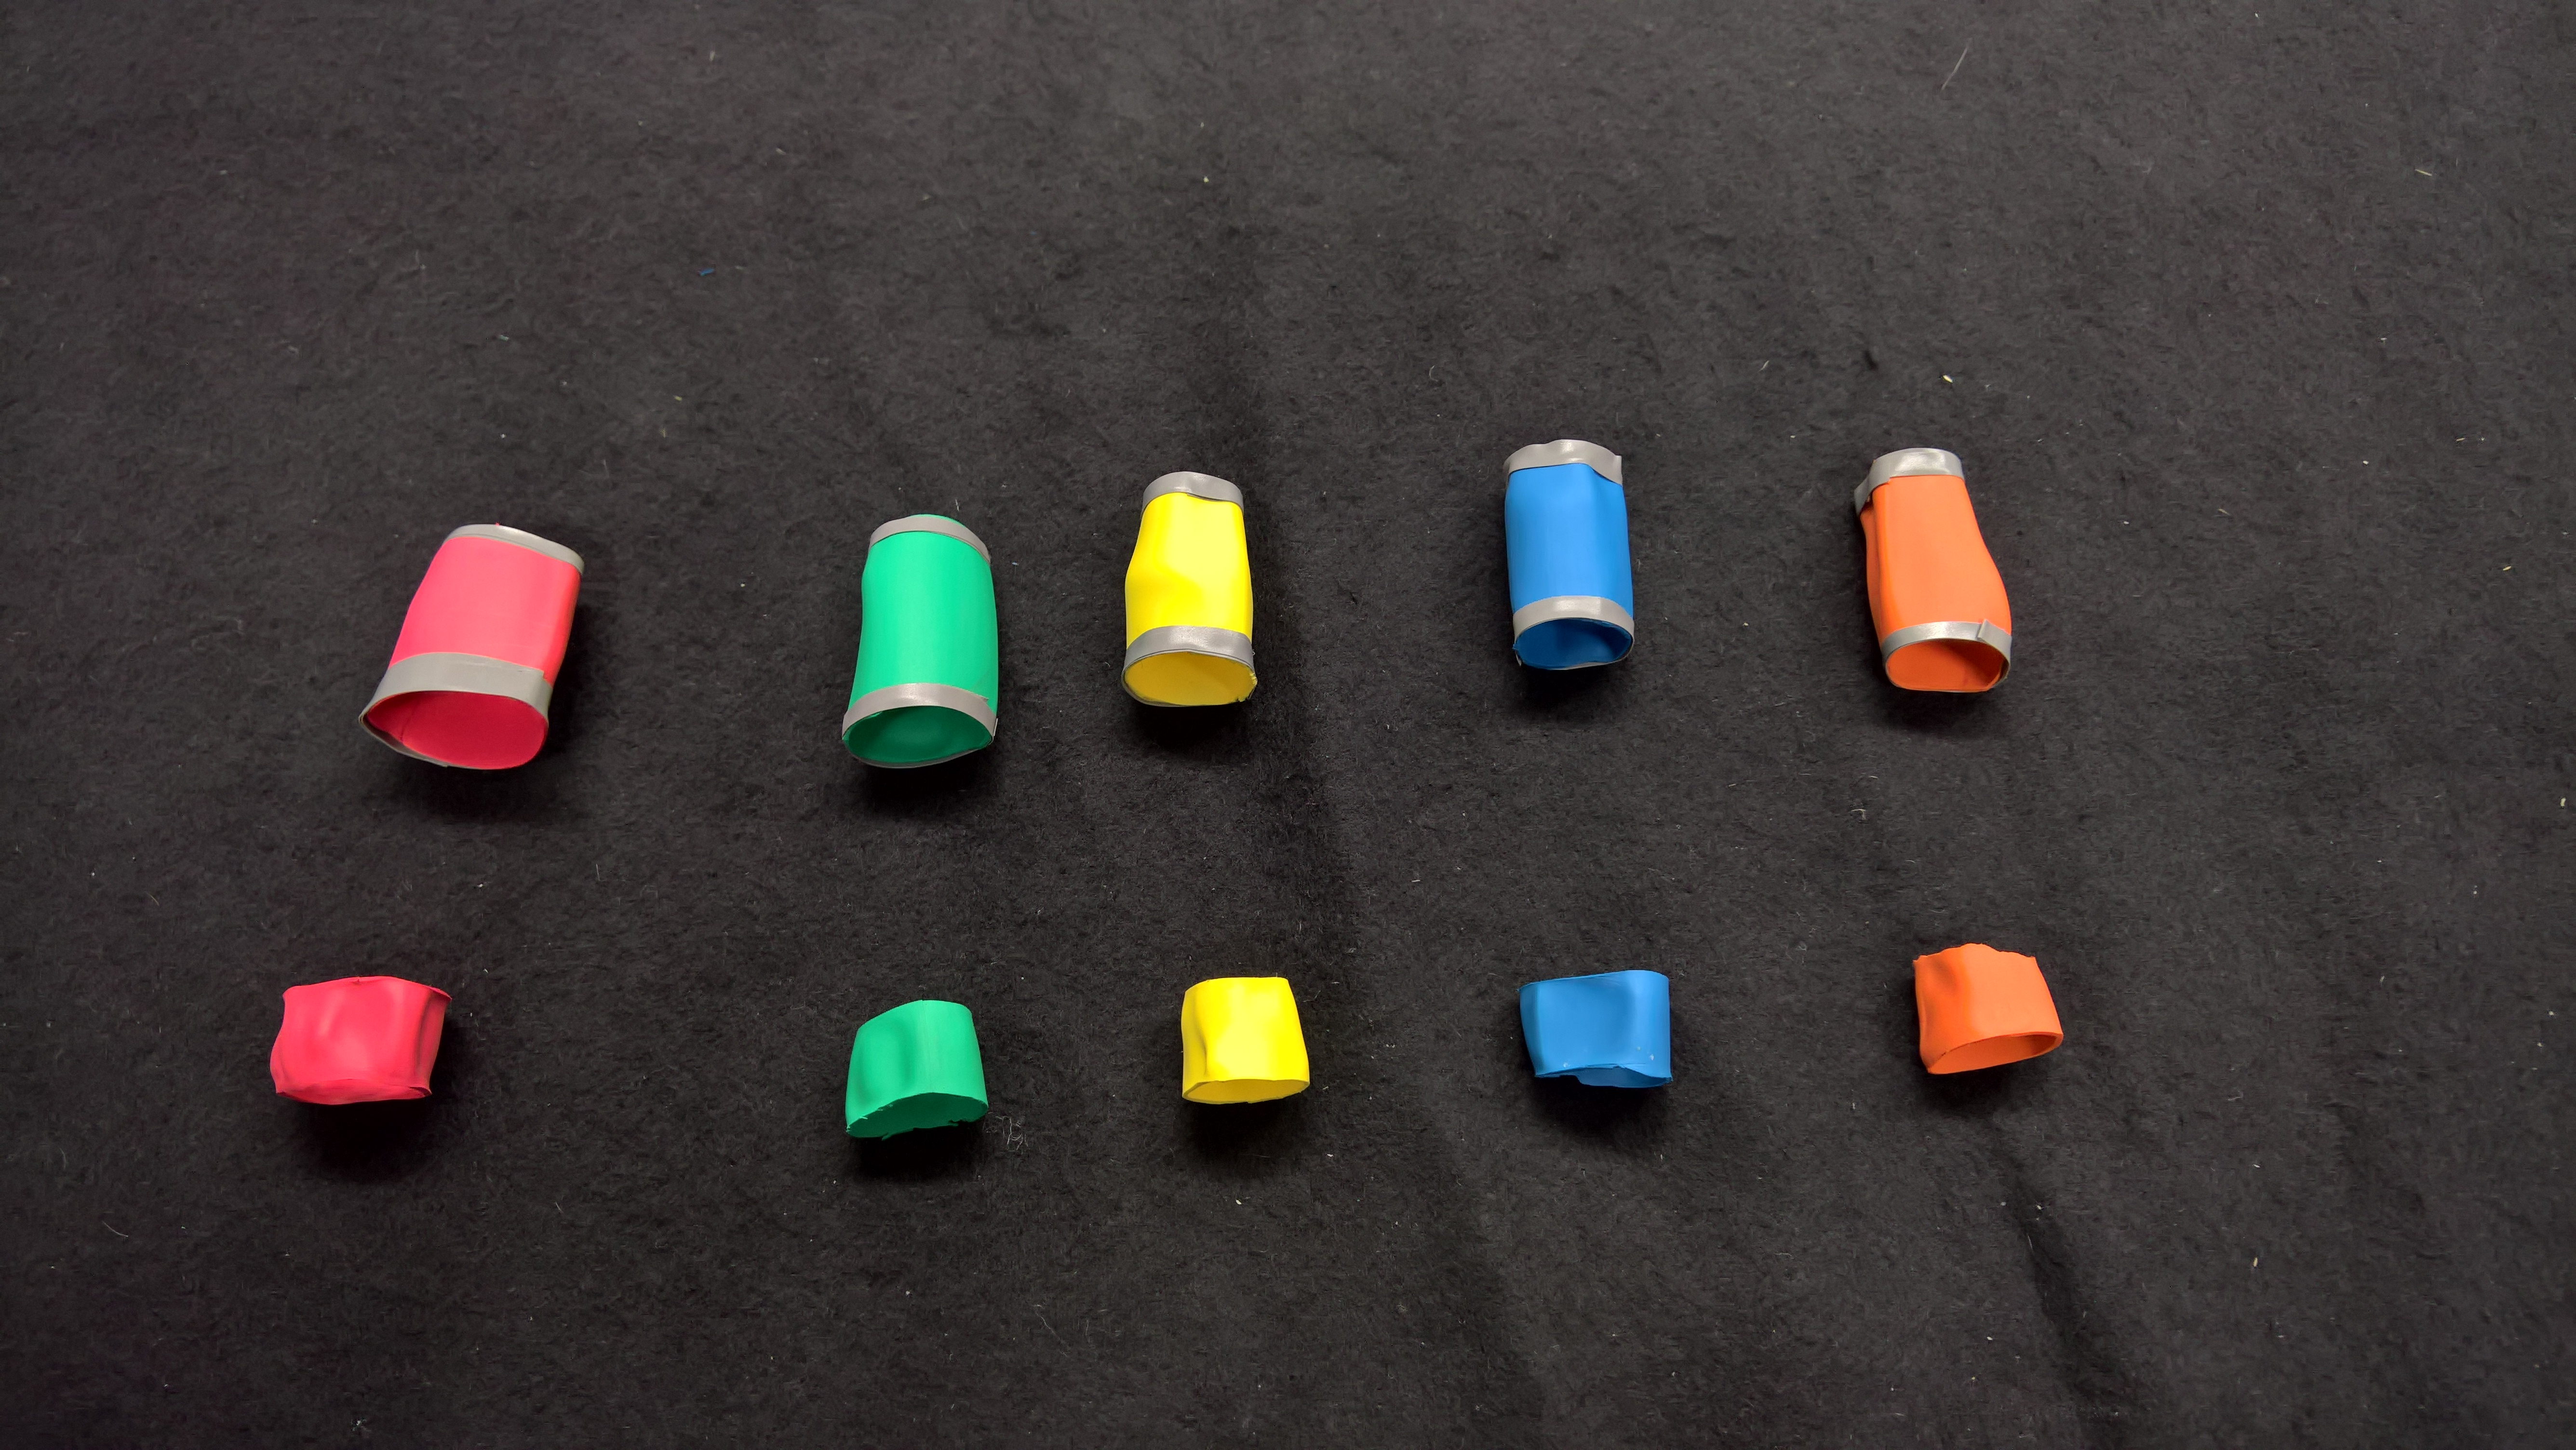
\includegraphics[width=0.5\textwidth]{images/small_and_improved_markers.jpg}
\caption{Improved larger and smaller set of shrink tube color markers }
\label{img:second_color_markers}
\end{figure}
The idea behind this solution was to create a fixed border between the color area of the tracker and the color area of the skin tones. The grey color of the border ensures that this area will not be tracked. The usage of black instead of gray would even furthermore ensure this. 
\\Since the threshold algorithm searches for the largest closed color area in the binary threshold image, this border should cause a separation of unwanted skin reflection area and actual tracker color area. The problem that the resulting color marker area might not be the largest area still persists after this improvement, but this case has to be handled separately.
\\\\Optical results showed that for the colors lying outside of the red to orange color spectrum that skin reflections produce, the artificial border stabilized the color detection.
\\The idea of using shrink tubing as marker material showed to be suitable except in the cases described above. One downside of the material is that the displayed colors are already the highest variety of available colors on the market. Other colors from the green and blue color areas like purple are simply not available or have to be ordered as a special request in larger amounts.
\\\\The original diameter is much larger than a human finger. The used shrink tube is able to be shrunken to one third of its size. The reason for this was to be able to adapt to the varying diameters of the human fingers. The shrinking procedure requires a constant amount of heat to be applied to the material to activate shrinking. The amount of heat that is needed surpasses the heat production of a standard hair dryer. The original application of shrink tubing is on heat resistant cables. The heat that needs to be applied can easily be more than 100 degree Celsius, which makes a direct application on the users hand highly insecure.
\\\\For the prototype, the shrink tube parts were shrunk with a standard cigarette lighter and continuously fitted onto the user finger until the desired form was reached. This method showed to  be sub-optimal, since the flame of the lighter produces only a punctual heat source. This caused uneven shrinkage of the heated parts. This can lead to cavities or bumps in the material. It  also changes the reflection properties at these points. A regulated heat gun would probably generate better results.
\\To get smoother shrinking results, parts of PVC tubing with the correct diameter could be used as dummy parts for the main part of the shrinking.\\
\\Another approach that was tested was the usage of matte acrylic paint to cover parts of the finger. The paint comes with the benefit of being easily to apply to the finger. Acrylic paint is available in much more color variations than the shrink tube. The finger coating is dry in under a minute after application. Adaption for finger size is automatically included in the application process. If the tracking system does not need to evaluate for hand rotation, i.e. the working principle is a top on view, a nail polish style application of the color on the fingernail can be sufficient for the tracking system. The thumb needs to be treated separately, as it has more rotation capabilities than the other fingers. It should be marked completely on all sides to achieve a constant tracking. If hand rotation is tracked, the other fingers should be completely marked as well.
\begin{figure}[H]
\centering
\includegraphics[width=0.5\textwidth]{images/final_finger_markers.jpg}
\caption{Finger marked with suitable acrylic colors}
\label{img:final_markers}
\end{figure}
\newpage As the final marker material, a mixture of blue and green color tones together with red tones in the purple and magenta section based on the acrylic color was chosen.
\begin{figure}[H]
\centering
\includegraphics[width=\textwidth]{images/acrylic_color_jitter.jpg}
\caption{Bar chart showing position jitter of final colors in static position}
\label{img:color_jitter}
\end{figure}
 The usage of the acrylic color also provides the least degradation in terms of haptics on the fingers. Figure \ref{img:color_jitter} shows the measured static position jitter of the system with the final colors. The reachable system precision lies between 2 and 5 pixel deviation. At a system resolution of 640x480 pixels, this results in a deviation of $\sim 0.7\%$ on the x axis and $\sim 1.0\%$ deviation on the y axis.
 \newpage
\subsection{Depth measurement accuracy}
To determine the accuracy of the system, the camera rig was aligned horizontally and fixed to a test bench. A large sized colored marker (75 mm x 50 mm) was used as tracking target. The marker was positioned at altering distances from the camera rig along the central axis. The height at which the camera rig is positioned in the experiment setup will be around 100 cm, so the measured distances started at 100 cm from the camera and were decremented in steps of 5 cm until 20 cm in front of the camera rig (see Table \ref{tbl:Depth measurement Values} and Figure \ref{char:DisparityToDistanceChart}).\\
\begin{figure}[H]
\includegraphics[width=\textwidth]{images/Disparity_to_distance.JPG}
\caption{Chart showing the results of the disparity measurement with a plotted trend line}
\label{char:DisparityToDistanceChart} 
\end{figure}
The accuracy of the camera system is limited by the number of pixels in relation to the camera view angle \cite{JernejMrovlje.2008}:\\
\begin{equation}
\Delta\varphi=\frac{\varphi_0}{x_0}
\end{equation}
\\
For the system setup of $x_{0}=$ 640 px image width and a horizontal view angle of $\varphi_{0}=62.5^\circ$, $\Delta\varphi$ is equal to $0.0977\frac{1^\circ}{pixel}$.\\\\
The resulting distance error would be:\\
\begin{equation}
\frac{\tan \varphi}{\tan(\varphi -\Delta\varphi)}=\frac{\Delta D+D}{D}
\end{equation}\\
\begin{equation}
\label{equ:delta_d}
\Delta D=\frac{D^{2}}{B} tan(\Delta\varphi)
\end{equation}
\\The system error for a target distance $D=100cm$ would therefore result in about $2cm$ of possible error.
As the measured values show deviations of up to $5\%$ from the correct value, the function from the fitted trend line displayed in Figure \ref{char:DisparityToDistanceChart} was taken as a correcting factor for the depth calculation.
\\\\Equation \ref{equ:delta_d} uses the uncorrected values for the calculation. Values lying on the trend line of Figure \ref{char:DisparityToDistanceChart} should correspond more to the correct distance values \cite{ManafA.Mahammed.2013}. The equation can be rewritten to:
\begin{equation}
\label{equ:power_function}
D=k*x^{z}
\end{equation}
with K being:
\begin{equation}
k=\frac{Bx_0}{2\tan(\frac{\varphi_0}{2}+\phi)}
\end{equation}
and \textit{x} the disparity in pixels.
The $\phi$ term in the equation above is used as a compensation for possible alignment errors.
The trend line, which is fit to the measurements in Figure \ref{char:DisparityToDistanceChart} represents the the function needed to fulfill Equation \ref{equ:power_function}. The calculated values are $k=4543.3$ and $z=-1.035$.
With the utilization of the corrected value formula, the accuracy of the depth measurement results is acceptable for the prototype application. For future work, the distance measurement procedure could be applied with more measurement points to refine the resulting function for more precision. The measurement values that were retrieved can be found in Table \ref{tbl:Depth measurement Values}.
\newpage
\begin{landscape}
\begin{table}[]
\label{char:Depth calibration measurement}
\centering
\caption{Depth measurement values}
\label{tbl:Depth measurement Values}
\begin{tabular}{|c|c|c|c|c|c|c|c|}
\hline
\begin{tabular}[c]{@{}c@{}}Real distance \\ from camera (cm)\end{tabular} & \begin{tabular}[c]{@{}c@{}}Left camera\\ x-value\end{tabular} & \begin{tabular}[c]{@{}c@{}}Right camera\\ x-value\end{tabular} & \begin{tabular}[c]{@{}c@{}}Disparity in\\  pixels\end{tabular} & \begin{tabular}[c]{@{}c@{}}Calculated distance\\ in cm\end{tabular} & Deviation in \%(abs.) & Corrected values & Deviation in \%(abs.) \\ \hline
100                                                                       & 302                                                           & 342                                                            & 40                                                             & 99.463                                                              & 0.54                  & 99.670           & 0.33                  \\ \hline
95                                                                        & 301                                                           & 343                                                            & 42                                                             & 94.727                                                              & 0.29                  & 94.760           & 0.25                  \\ \hline
90                                                                        & 300                                                           & 344                                                            & 44                                                             & 90.421                                                              & 0.47                  & 90.304           & 0.34                  \\ \hline
85                                                                        & 298                                                           & 346                                                            & 48                                                             & 82.886                                                              & 2.49                  & 82.523           & -2.91                 \\ \hline
80                                                                        & 296                                                           & 345                                                            & 49                                                             & 81.194                                                              & 1.49                  & 80.780           & 0.98                  \\ \hline
75                                                                        & 296                                                           & 348                                                            & 52                                                             & 76.510                                                              & 2.01                  & 75.960           & 1.28                  \\ \hline
70                                                                        & 293                                                           & 349                                                            & 56                                                             & 71.045                                                              & 1.49                  & 70.349           & 0.5                   \\ \hline
65                                                                        & 289                                                           & 350                                                            & 61                                                             & 65.222                                                              & 0.34                  & 64.388           & 0.94                  \\ \hline
60                                                                        & 289                                                           & 355                                                            & 66                                                             & 60.281                                                              & 0.47                  & 59.344           & 1.09                  \\ \hline
55                                                                        & 286                                                           & 357                                                            & 71                                                             & 56.036                                                              & 1.88                  & 55.022           & 0.04                  \\ \hline
50                                                                        & 285                                                           & 361                                                            & 76                                                             & 52.349                                                              & 4.7                   & 51.279           & 2.56                  \\ \hline
45                                                                        & 280                                                           & 365                                                            & 85                                                             & 46.806                                                              & 4.01                  & 45.668           & 1.48                  \\ \hline
40                                                                        & 265                                                           & 362                                                            & 97                                                             & 41.016                                                              & 2.54                  & 39.831           & 0.42                  \\ \hline
35                                                                        & 258                                                           & 367                                                            & 109                                                            & 36.5                                                                & 4.29                  & 35.300           & 0.86                  \\ \hline
30                                                                        & 244                                                           & 373                                                            & 129                                                            & 30.841                                                              & 2.80                  & 29.650           & 1.17                  \\ \hline
25                                                                        & 288                                                           & 381                                                            & 153                                                            & 26.003                                                              & 4.01                  & 24.848           & 0.61                  \\ \hline
20                                                                        & 206                                                           & 395                                                            & 189                                                            & 21.050                                                              & 5.25                  & 19.965           & 0.17                  \\ \hline
\end{tabular}

\end{table}
\end{landscape}
\section{Data filtering}
The finger marker base jitter measurements showed that the systems can only supply a certain stability of position tracking. This results in the fluctuation of the measurement results. When rendering this unfiltered data directly, a large optical jitter in all positions is the case. Jittering of position values also causes the height calculation algorithm to generate incorrect height values.\\
To counter this data jitter, the incoming data-set is filtered on the "Master" in several steps with the \textit{1 euro filter} presented by Casiez et al. \cite{Casiez.2012}. It uses a first order low-pass filter with an adaptive cutoff frequency to filter noisy signals for high precision and responsiveness. This means that at low speeds, a low cutoff reduces jitter at the expense of lag. At high speeds, the cutoff is increased to reduce lag rather than jitter.\\
The filter was chosen, beacuase of a relative simple and easy implementation as well as an uncomplicated setup and tuning process. It also produces faster and better results in comparsion to the normally used \textit{Kalman filter} \cite{Welch.2001}, \textit{moving average filter} or \textit{low-pass filters and exponential smoothing filters} \cite{LaViola.2003}.\\ The filter needs three base values to function correctly. The first one is the frequency at which the data values are delivered. This can easily be measured from the time stamp differences of the incoming data packages. The other two values are the minimum cutoff frequency$f_{c_{min}} $ of the low pass filter and the slope of the filter curve $\beta$.
\\These values have to be calibrated in a manual process for each marker. In the first step the value of $f_{c_{min}} $ is set to one and $\beta$ is set to zero. The markers are held in a static position or moved very slowly to check for jitter. The value of $f_{c_{min}} $ is then adapted to a point where the jitter is minimized without creating to much lag for these slow movements. In the second step, the tracker is moved fast and the $\beta$ value is increased until lag for fast movements is minimized.
\\\\ In a first step, the incoming data for each finger and the base marker are filtered separately and component-wise. This allows for specific fine tuning of the filter values, as each marker shows different jitter. The incoming values are also passed to the depth calculation algorithm where the z position of the respective marker is calculated. The result is also filtered before all components are written into the final result position vector.\\
The individual filter application to all values resulted in a much smoother and less jittering optical result in comparison to the raw tracking values.
\newpage
\section{Inverse kinematics algorithm}
Figure \ref{img:hand-constraint_debug_view} shows the a debugging representation of the used kinematic structure of the \textit{Caliko} framework. The non-black colored lines of the left picture show the kinematic chains for each finger. The black colored lines are used as an offset structure from the hand base marker.
The kinematic chains all have their own target point for which the algorithm can solve for. All chains are grouped into a kinematic model for easier data handling. The kinematic model provides a container for easier access of the base and the connection structure through which the fingers are connected to the base.
With this data, the algorithm is capable of calculating a solution for each kinematic finger chain and applying these values to the position. If the target is reachable, the digital finger position should match the pose of its real world counterpart up to a specified threshold value.
\begin{figure}[H]
\centering
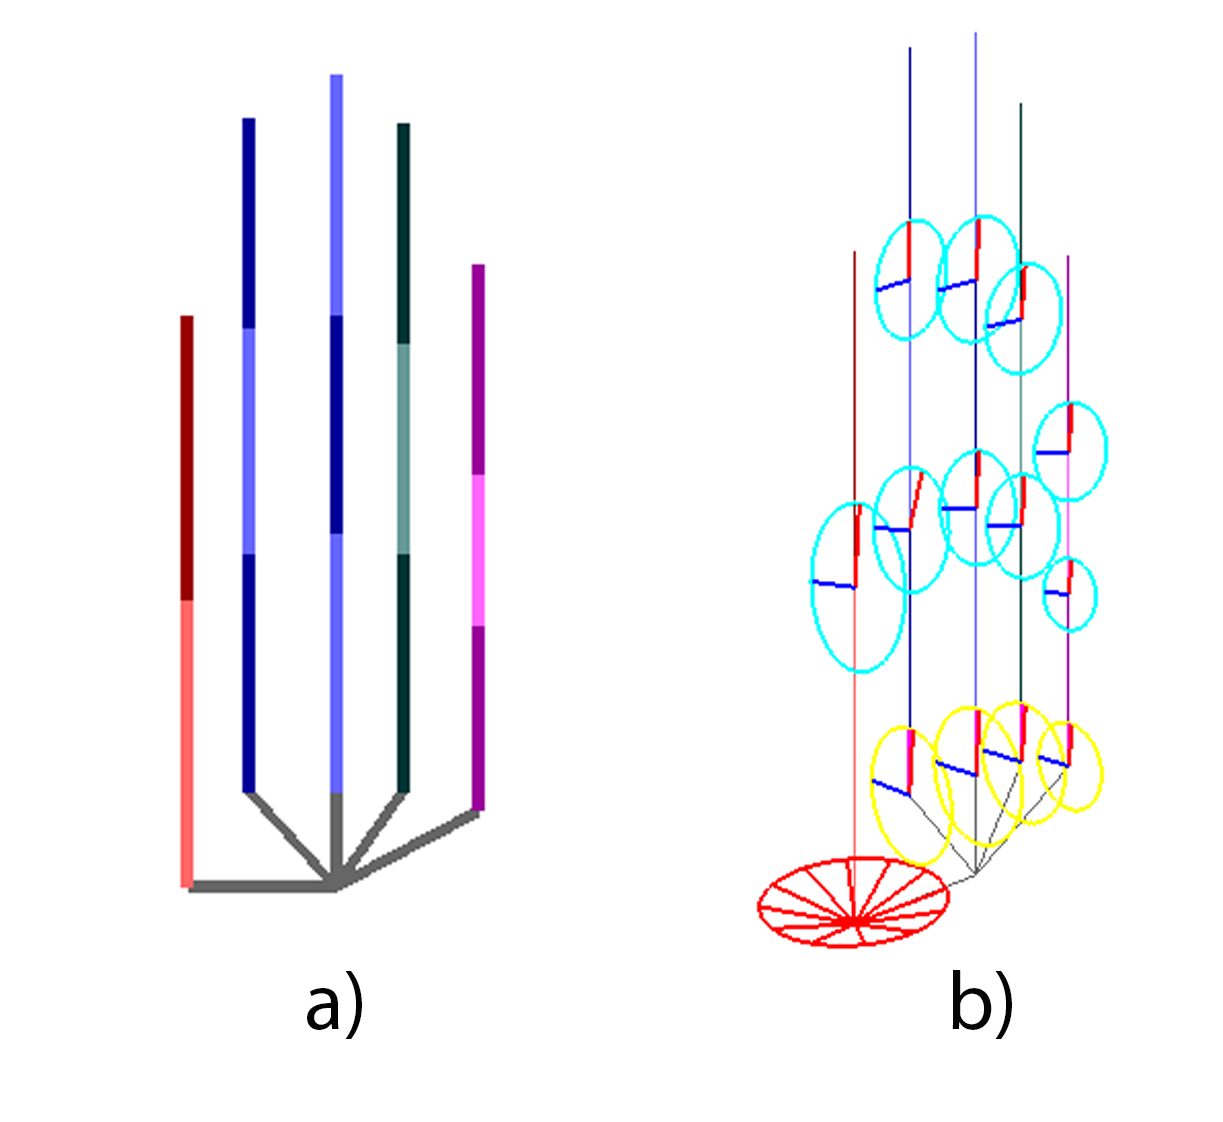
\includegraphics[width=0.5\textwidth]{images/hand_model_combo.png}
\caption{Hand model representation of the used IK framework: a) Kinematic chains and base structure, b) Hand model with visualized movement constraints}
\label{img:hand-constraint_debug_view} 
\end{figure}
The right image shows the same model with applied constraints to each chains. The framework differentiates between base-bone constraints and normal bone constraints. The base-bone constraints are treated separately as the base-bone is the starting point of the kinematic chain and therefore effects all following bones. In the 3D mode constraints with either a global or a local reference axis can be applied. The local reference axis usually refers to a axis of the previous bone. Global constraints are used for base-bone constraints. The reference axis can the be used for the specific type of constraint. The framework supports hinge type constraints and rotor constraints. The hinge types define a rotation axis around which the bone can rotate (1 DOF). The rotor-based constraint defines an angle for a cone on a defined axis which limits the movement of the joint in multiple directions (2 DOF). This circular curve limitation is a downside of the framework as a parabolic curve description for a rotor-based constraint would better fit the movement capabilities of the fingers.
\newpage 
\section{Grabbing test}
To test the tracking limitations of the system , a grabbing test with the tracked \textit{HTC Vive} marker and the tracked hand was done.
Before the test was started, it was ensured that the infrared signals from the object tracker do not interfere with the camera images for tracking. 
\begin{figure}[H]
\centering
\includegraphics[width=0.8\textwidth]{images/occlusion_set.jpg}
\caption{Grabbing test results: Upper image pair shows grabbing of tracker without finger occlusion. The position of the hand and the fingers is correct. The bottom image pair shows the mentioned marker occlusion problem. The tracker  position is correct but the finger tracking is lost and the positoin of the hand incorrect.}
\label{img:hand_rendering}
\end{figure}
The built-in infrared filters of the camera manage to filter out the signals, as no image distortion was visible. The test chore was to pick up the tracked marker based on the position of the marker representation in digital space.
A precise initial position calibration for the object tracker is done to ensure matching real and digital positions. The tracking limitations of the system showed when bending the fingers around the marker to pick it up. The bending causes the fingers to be occluded from the cameras and no new position can be tracked. This occlusion problem results from the positioning of the cameras. The top-down view limits the movement areas of the hand where all fingers markers can be tracked. The hand position marker is not affected from this occlusion problem as long as the hand is not turned around.
For the system to handle grabbing movements correctly, the cameras would have to be positioned at a different angle than the top down-view or a further pair of cameras recording from a different angle has to be added.
